\label{Figure Data Augmentation}
\begin{figure}[H]
    \centering
    \begin{subfigure}{0.15\textwidth}
        \centering
        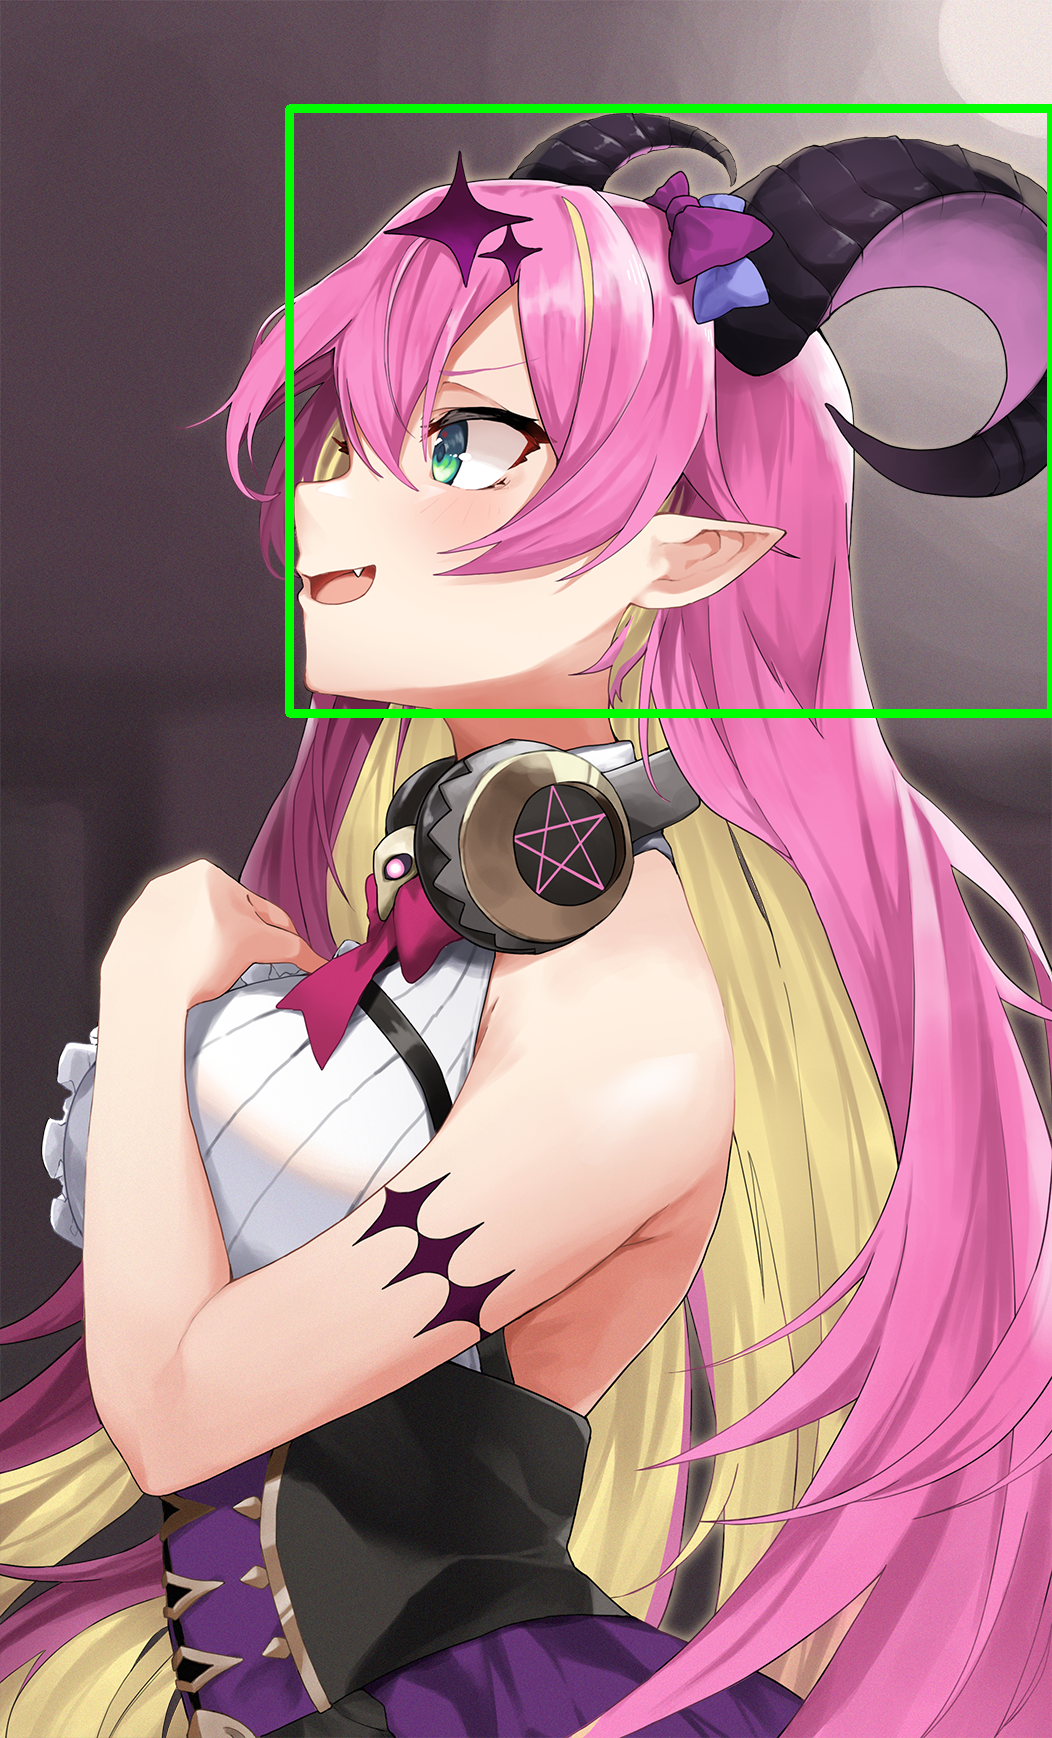
\includegraphics[width=\textwidth]{images/augmentation/Pixiv-83768702_p0-BB.png}
        \caption{}
        \label{fig:aloe1}
    \end{subfigure}
    \hfill
    \begin{subfigure}{0.15\textwidth}
        \centering
        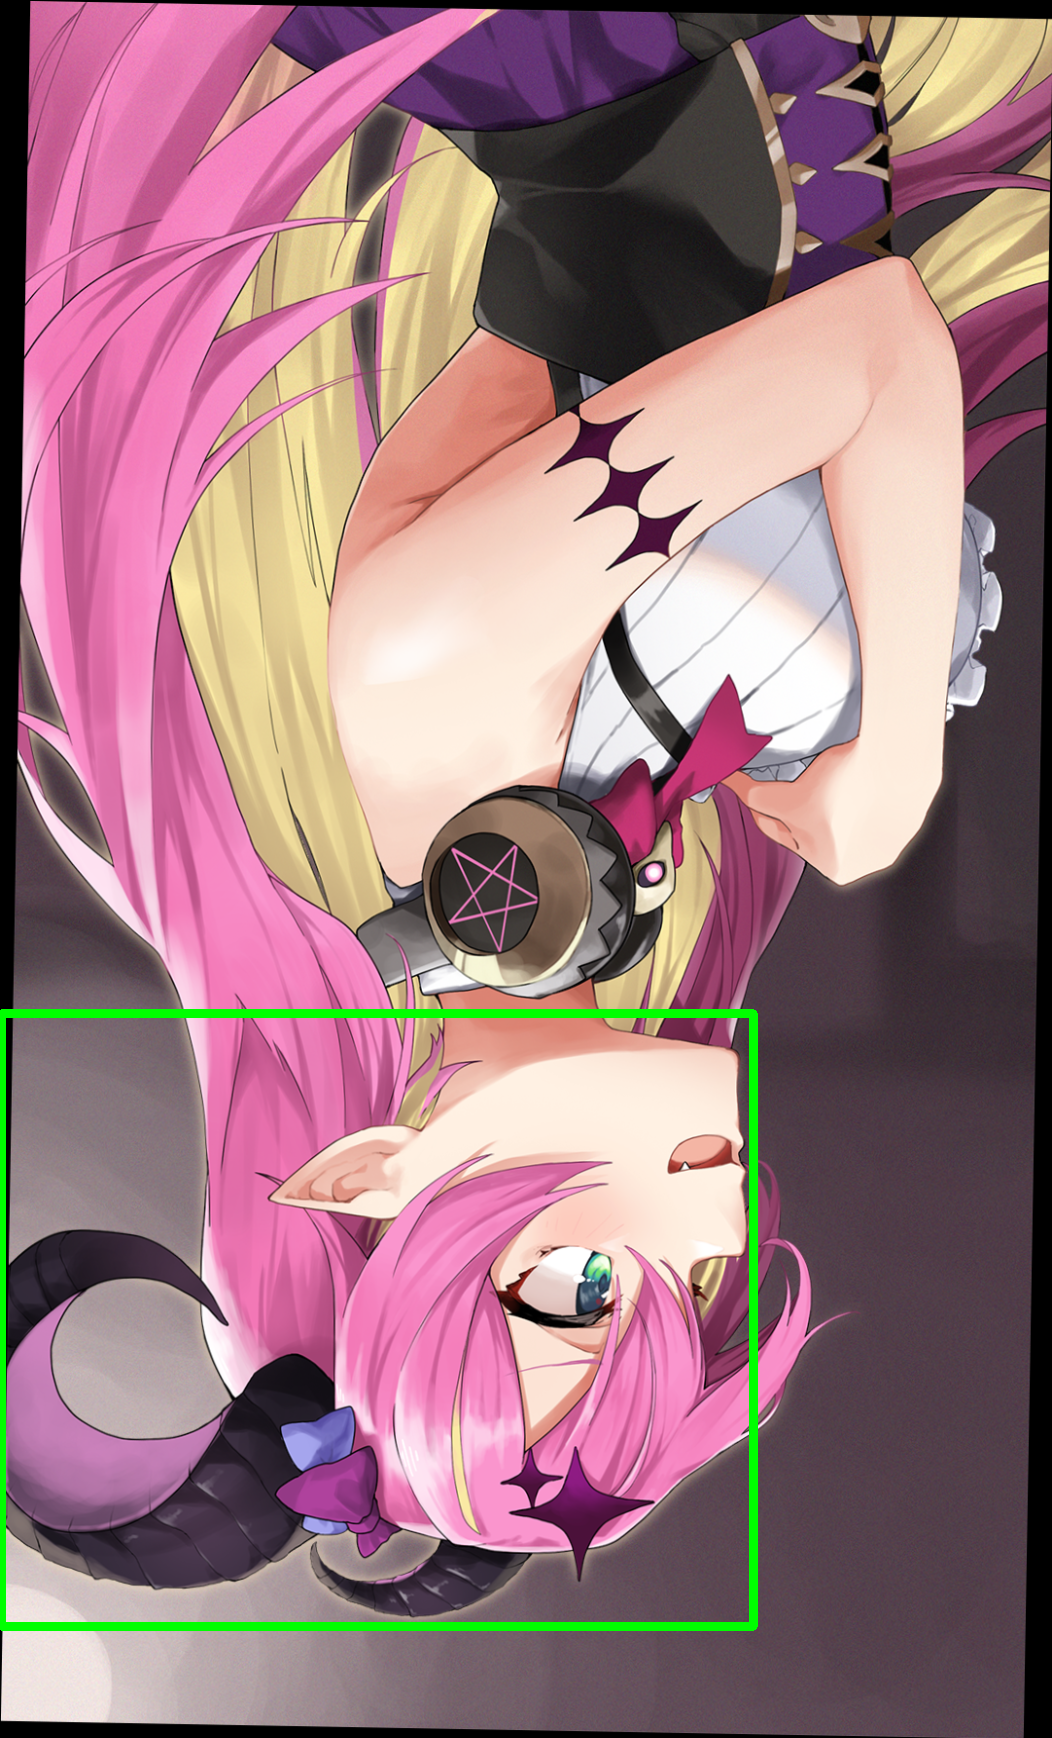
\includegraphics[width=\textwidth]{images/augmentation/Pixiv-83768702_p0-RandomRotate_179-BB.png}
        \caption{}
        \label{fig:aloe2}
    \end{subfigure}
    \hfill
    \begin{subfigure}{0.15\textwidth}
        \centering
        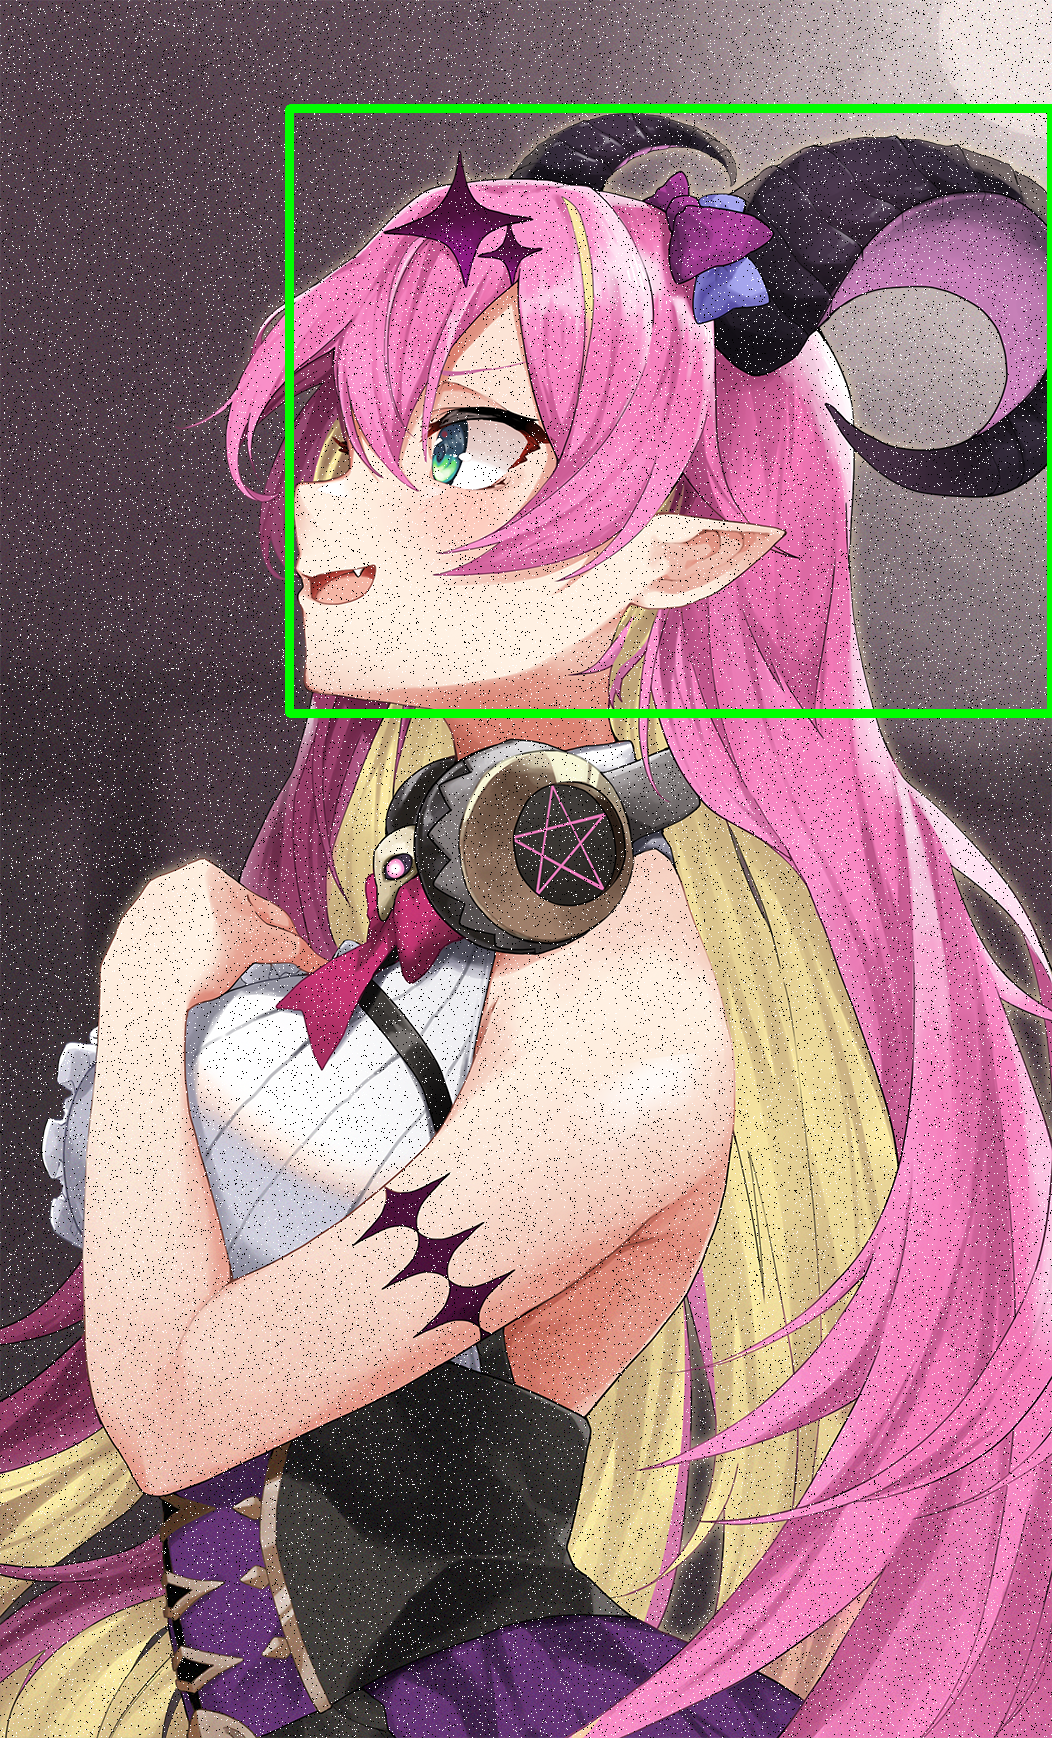
\includegraphics[width=\textwidth]{images/augmentation/Pixiv-83768702_p0-RandomSaltAndPepper_0.044-BB.png}
        \caption{}
        \label{fig:aloe3}
    \end{subfigure}
    \hfill
    \begin{subfigure}{0.15\textwidth}
        \centering
        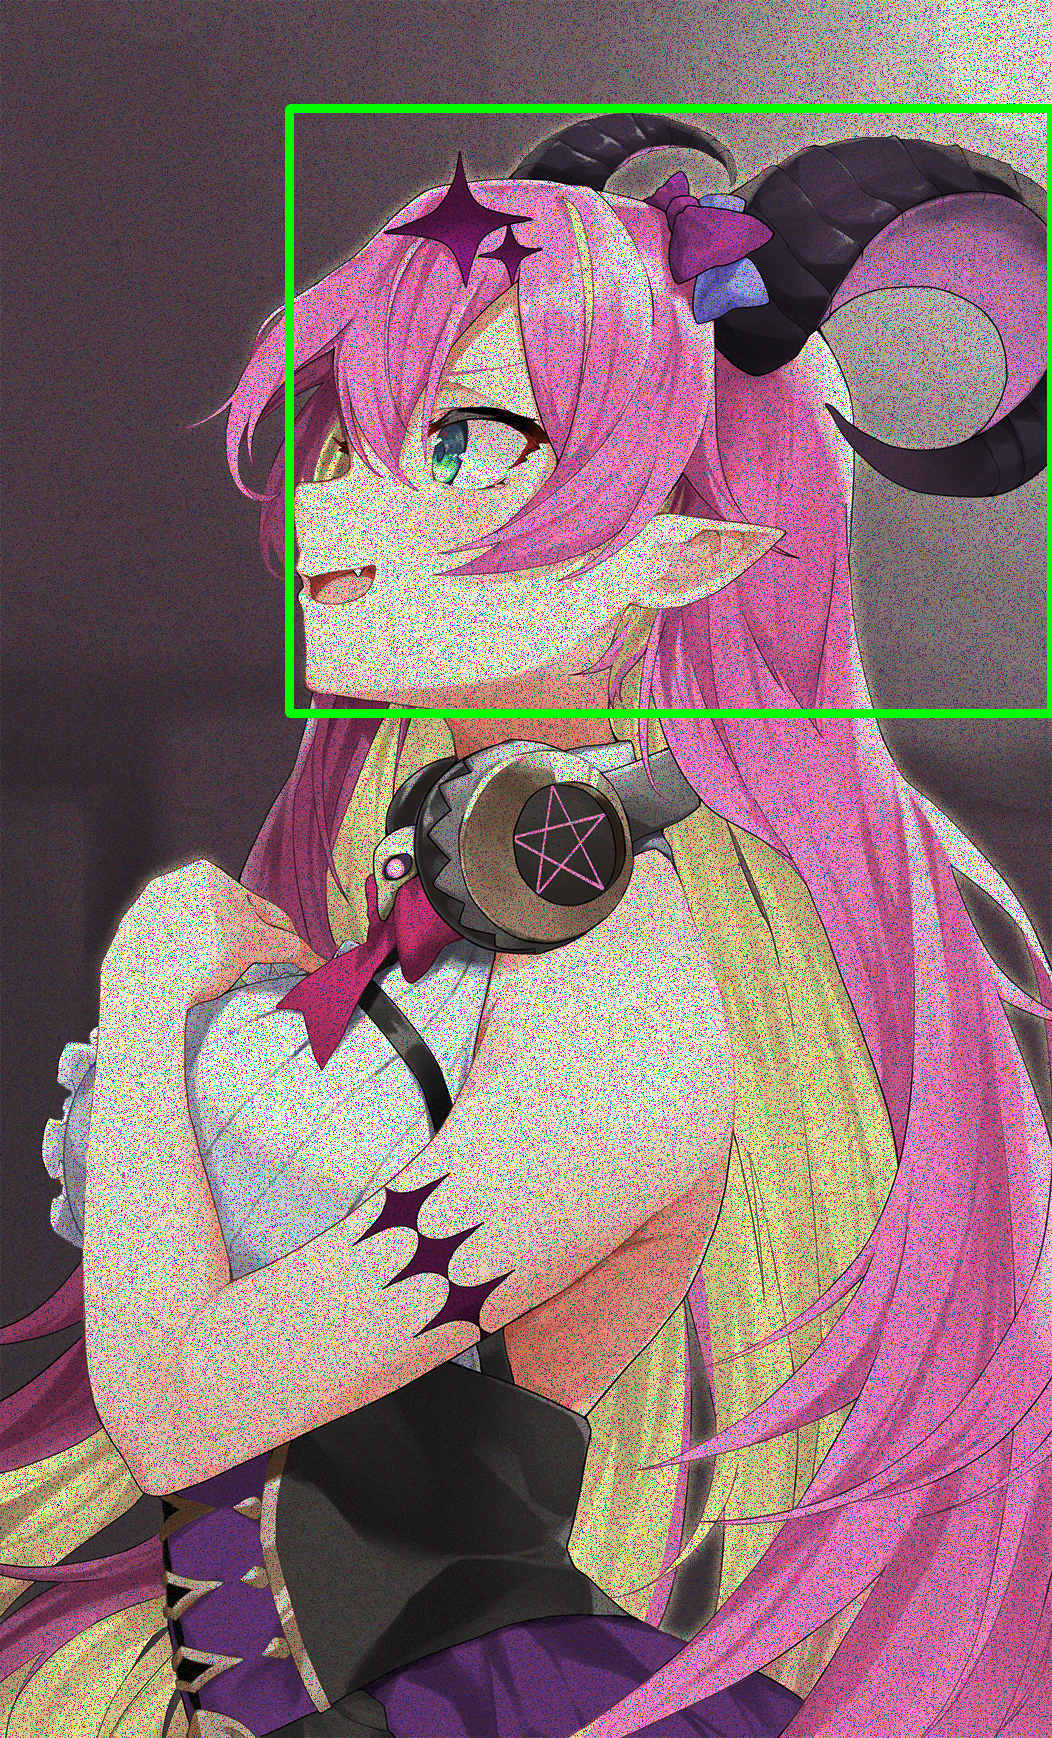
\includegraphics[width=\textwidth]{images/augmentation/Pixiv-83768702_p0-RandomValuedImpulseNoise_0.138-BB.png}
        \caption{}
        \label{fig:aloe4}
    \end{subfigure}
    \begin{subfigure}{0.15\textwidth}
        \centering
        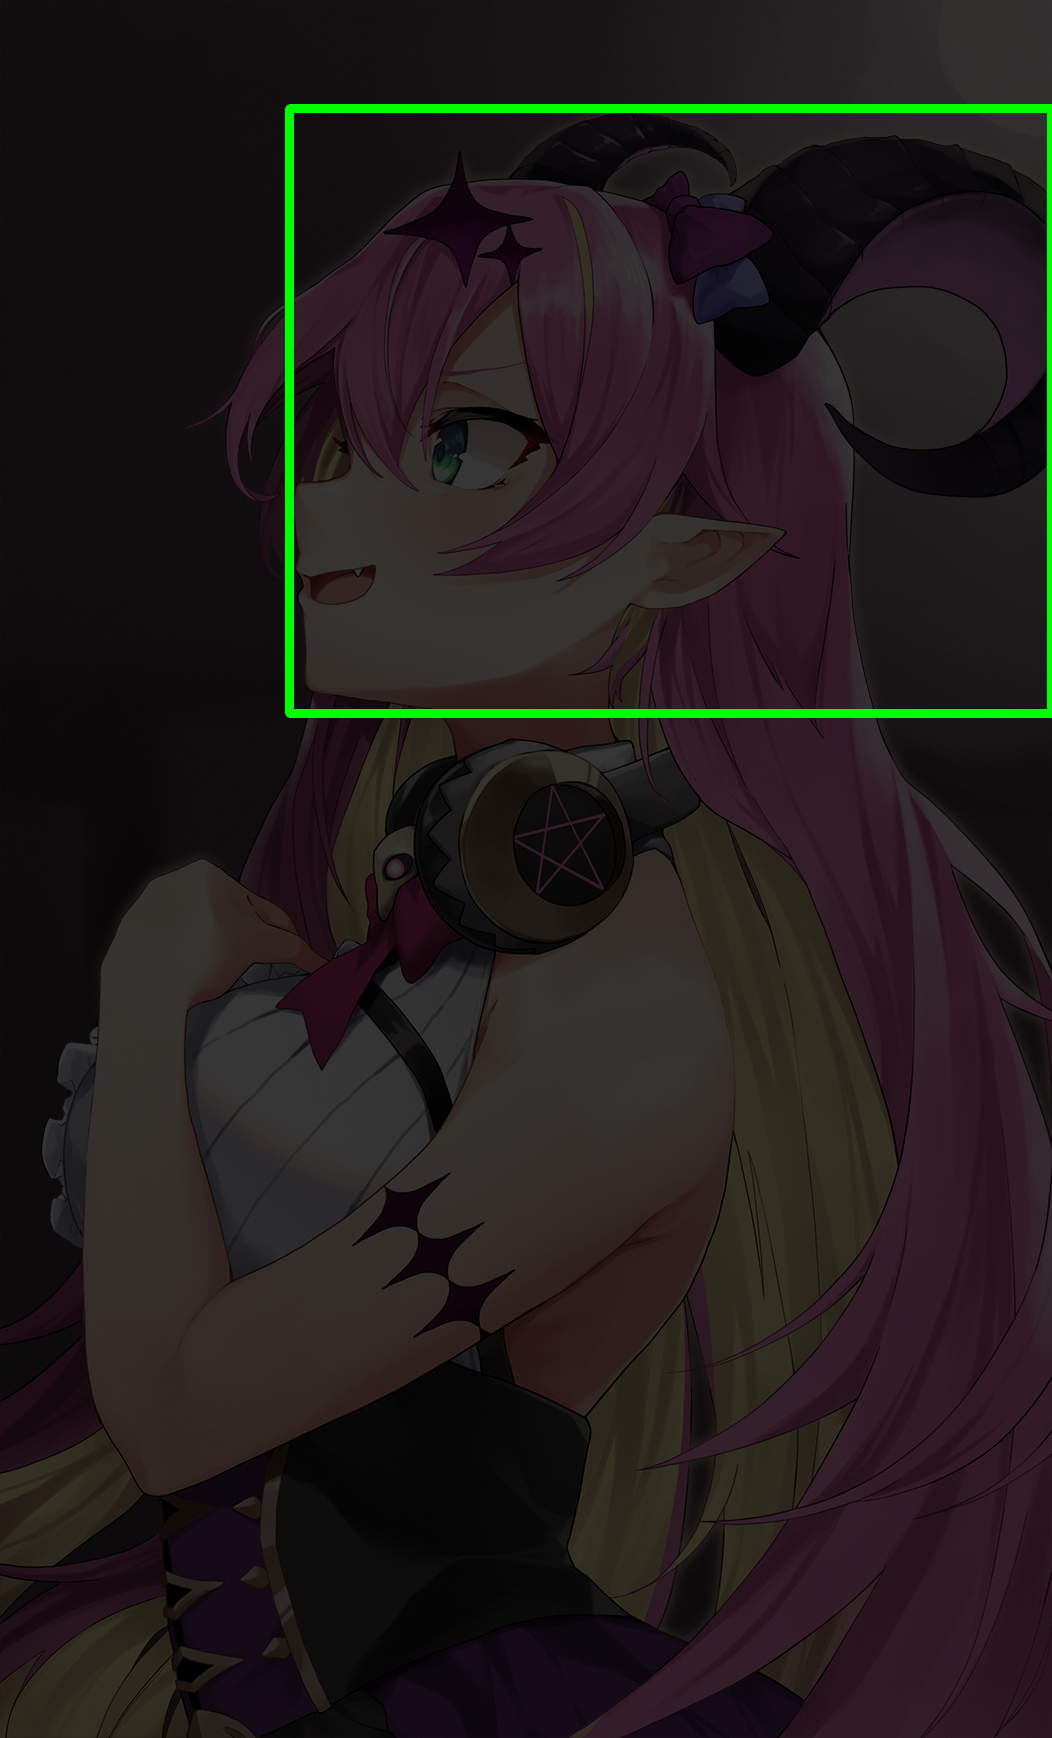
\includegraphics[width=\textwidth]{images/augmentation/Pixiv-83768702_p0-RandomBrightness_0.213-BB.png}
        \caption{}
        \label{fig:aloe5}
    \end{subfigure}
    \begin{flushleft}
        (a) Original image\cite{83768702}\\
        (b) Rotate 179 degrees\\
        (c) Random Salt and Pepper with 4.4\% \\
        (d) Random Valued Impulse Noise with 13.8\% \\
        (e) Brightness with intensity 0.213\\
    \end{flushleft}
    \caption{Data augmentation methods}
    \label{fig:manoaloe1}
\end{figure}